\documentclass[a4paper,11pt]{article}

\usepackage{graphicx}
% Set path for figure inputs
\graphicspath{{../output/figures/}}
% Set path for tables input
\makeatletter
\def\input@path{{../output/tables/}}
\makeatother

\usepackage{array}
\usepackage{caption}
\usepackage{graphicx}
\usepackage{colortbl}
\usepackage{siunitx}
\usepackage[normalem]{ulem}
\usepackage{colortbl}
\usepackage{multirow}
\usepackage{hhline}
\usepackage{calc}
\usepackage{tabularx}
\usepackage{threeparttable}
\usepackage{wrapfig}
\usepackage{adjustbox}
\usepackage{url}
\usepackage{apacite} 				
\usepackage{natbib}	
\setcitestyle{round,aysep={}}
\usepackage{amsmath}
\usepackage{amssymb} 
\usepackage{lmodern}
\usepackage{float}

\usepackage{geometry}
\geometry{a4paper,left=2.5cm,right=2.5cm,top=2.5cm,bottom=2.5cm}

\usepackage{hyperref}
\hypersetup{
	pdfauthor = {},
	pdftitle = {RIA Report},
	pdfkeywords = {},
	linkcolor=black,
    filecolor=blue,  
    citecolor=blue,
    urlcolor=cyan,
}
\linespread{1.3}
\begin{document}
\title{An Ex-Post Assessment of the ASEAN-China Free Trade Agreement (ACFTA) \\ Estimates Based on a Gravity Model}
\author{Linh Bui, Gero Dasbach, Shanawar Rana\thanks{We are thankful to Prof. Dr. Bruno Merlevede for helpful theoretical insights and Dr. Ruben Dewitte for his valuable guidance along all steps towards finishing this report.}}
\date{\today}
\maketitle
\begin{abstract}
\noindent Using BACI data on bilateral trade flows, we analyse the effects of trade liberalisation of the ASEAN-China Free Trade Agreement (ACFTA) on trade creation and trade diversion. Employing a gravity framework, we are able to obtain estimates for trade flows relative to the normal level for four different pairs of countries. We find that ACFTA boosts trade within ACFTA member countries, as well as trade with countries sharing an FTA with ACFTA countries. Moreover, trade increases between countries exporting to and importing from ACFTA. Our results in line with the idea of pure trade creation, we find no evidence for a Viner ambiguity.  \\ \\
\noindent \textbf{Keywords: } ACFTA, Economic Integration, Trade, Tariffs, Gravity Model, Trade Creation, Trade Diversion\\
\end{abstract}

\newpage

\begin{section}{Introduction}
Since the early 1990s, significant progress has been made in regional integration in the most important economic areas in the world. As bilateral and regional trade liberalization is becoming increasingly prominent, it is crucial to ascertain what implications this may have for world trade.

This study will focus on the ASEAN-CHINA Free Trade Agreement Asian (hereafter named "ACFTA"). ASEAN countries and China have been involved in market integration and have gained fame as the “world factory.” Hence, studying the impact of ACFTA will contribute to empirical evidence on the regional integration and international trade flows. 

Any assessment of the trade effects stemming from the formation of free trade agreements is always accompanied by the concepts of trade creation and trade diversion, which were first introduced by \cite{viner1950}.

Trade creation occurs when new trade arises between member countries due to reduced internal trade barriers. Trade diversion emerges when imports from a higher-cost member country replace imports from a low-cost extra-bloc country because the intra-bloc country has preferential access to the market and does not have to pay tariffs. Thus, the results of trade creation in an improvement in resource allocation presumably have positive welfare effects. Conversely, trade diversion refers to a welfare loss caused by a shift in the origin of a product from an extra-bloc producer (\citeauthor{carrere_2006}, 2006).

The formation of ACFTA helps ASEAN members to access the prosperous Chinese market and fosters economic growth in ASEAN countries. Meanwhile, ACFTA provides China with opportunities to obtain more raw materials to be used in production and helps Chinese enterprises extend their foreign market in Southeast Asia. Generally, ACFTA can be expected to have significant trade creation effects, which means a positive trade effect overall.

This study aims to evaluate the trade creation and diversion effects of the free trade agreements between ASEAN and China. The main research question is by how much trade creation and trade diversion between China and the ASEAN countries change after the introduction of FTA?

The rest of the paper is organised as follows. Section 2 presents a literature review including the evolution of trade between China and ASEAN, theoretical foundations and empirical evidence related to ex-Post assessment of regional trade agreement. Section 3 explains the model specification, our hypotheses and data. Section 4 reports the empirical results. Finally, Section 5 concludes.

\end{section}

\begin{section}{Literature Review}

\begin{subsection}{Evolution of Trade Between China and ASEAN}

China’s accession to the WTO in 2001 marked an important new opportunity to forge closer economic ties around the world. The idea to adopt a ACFTA between ASEAN member states and China was first voiced at the ASEAN-China summit on 6 November 2001. On 4 November 2002, China and ASEAN Countries signed the New Framework Agreement on Comprehensive Economic Cooperation (hereafter named "the Agreement") which formed the legal basis for the creation of the ACFTA (\cite{asean_2002_1}). In order to interpret the evolution of trade flows shown in \autoref{fig_1}, it is worthwhile to consult the Agreement. Policymakers aimed at stimulating trade between ASEAN and China through the reduction of both tariff- and non-tariff barriers.

\begin{figure}[H]
	\centering
	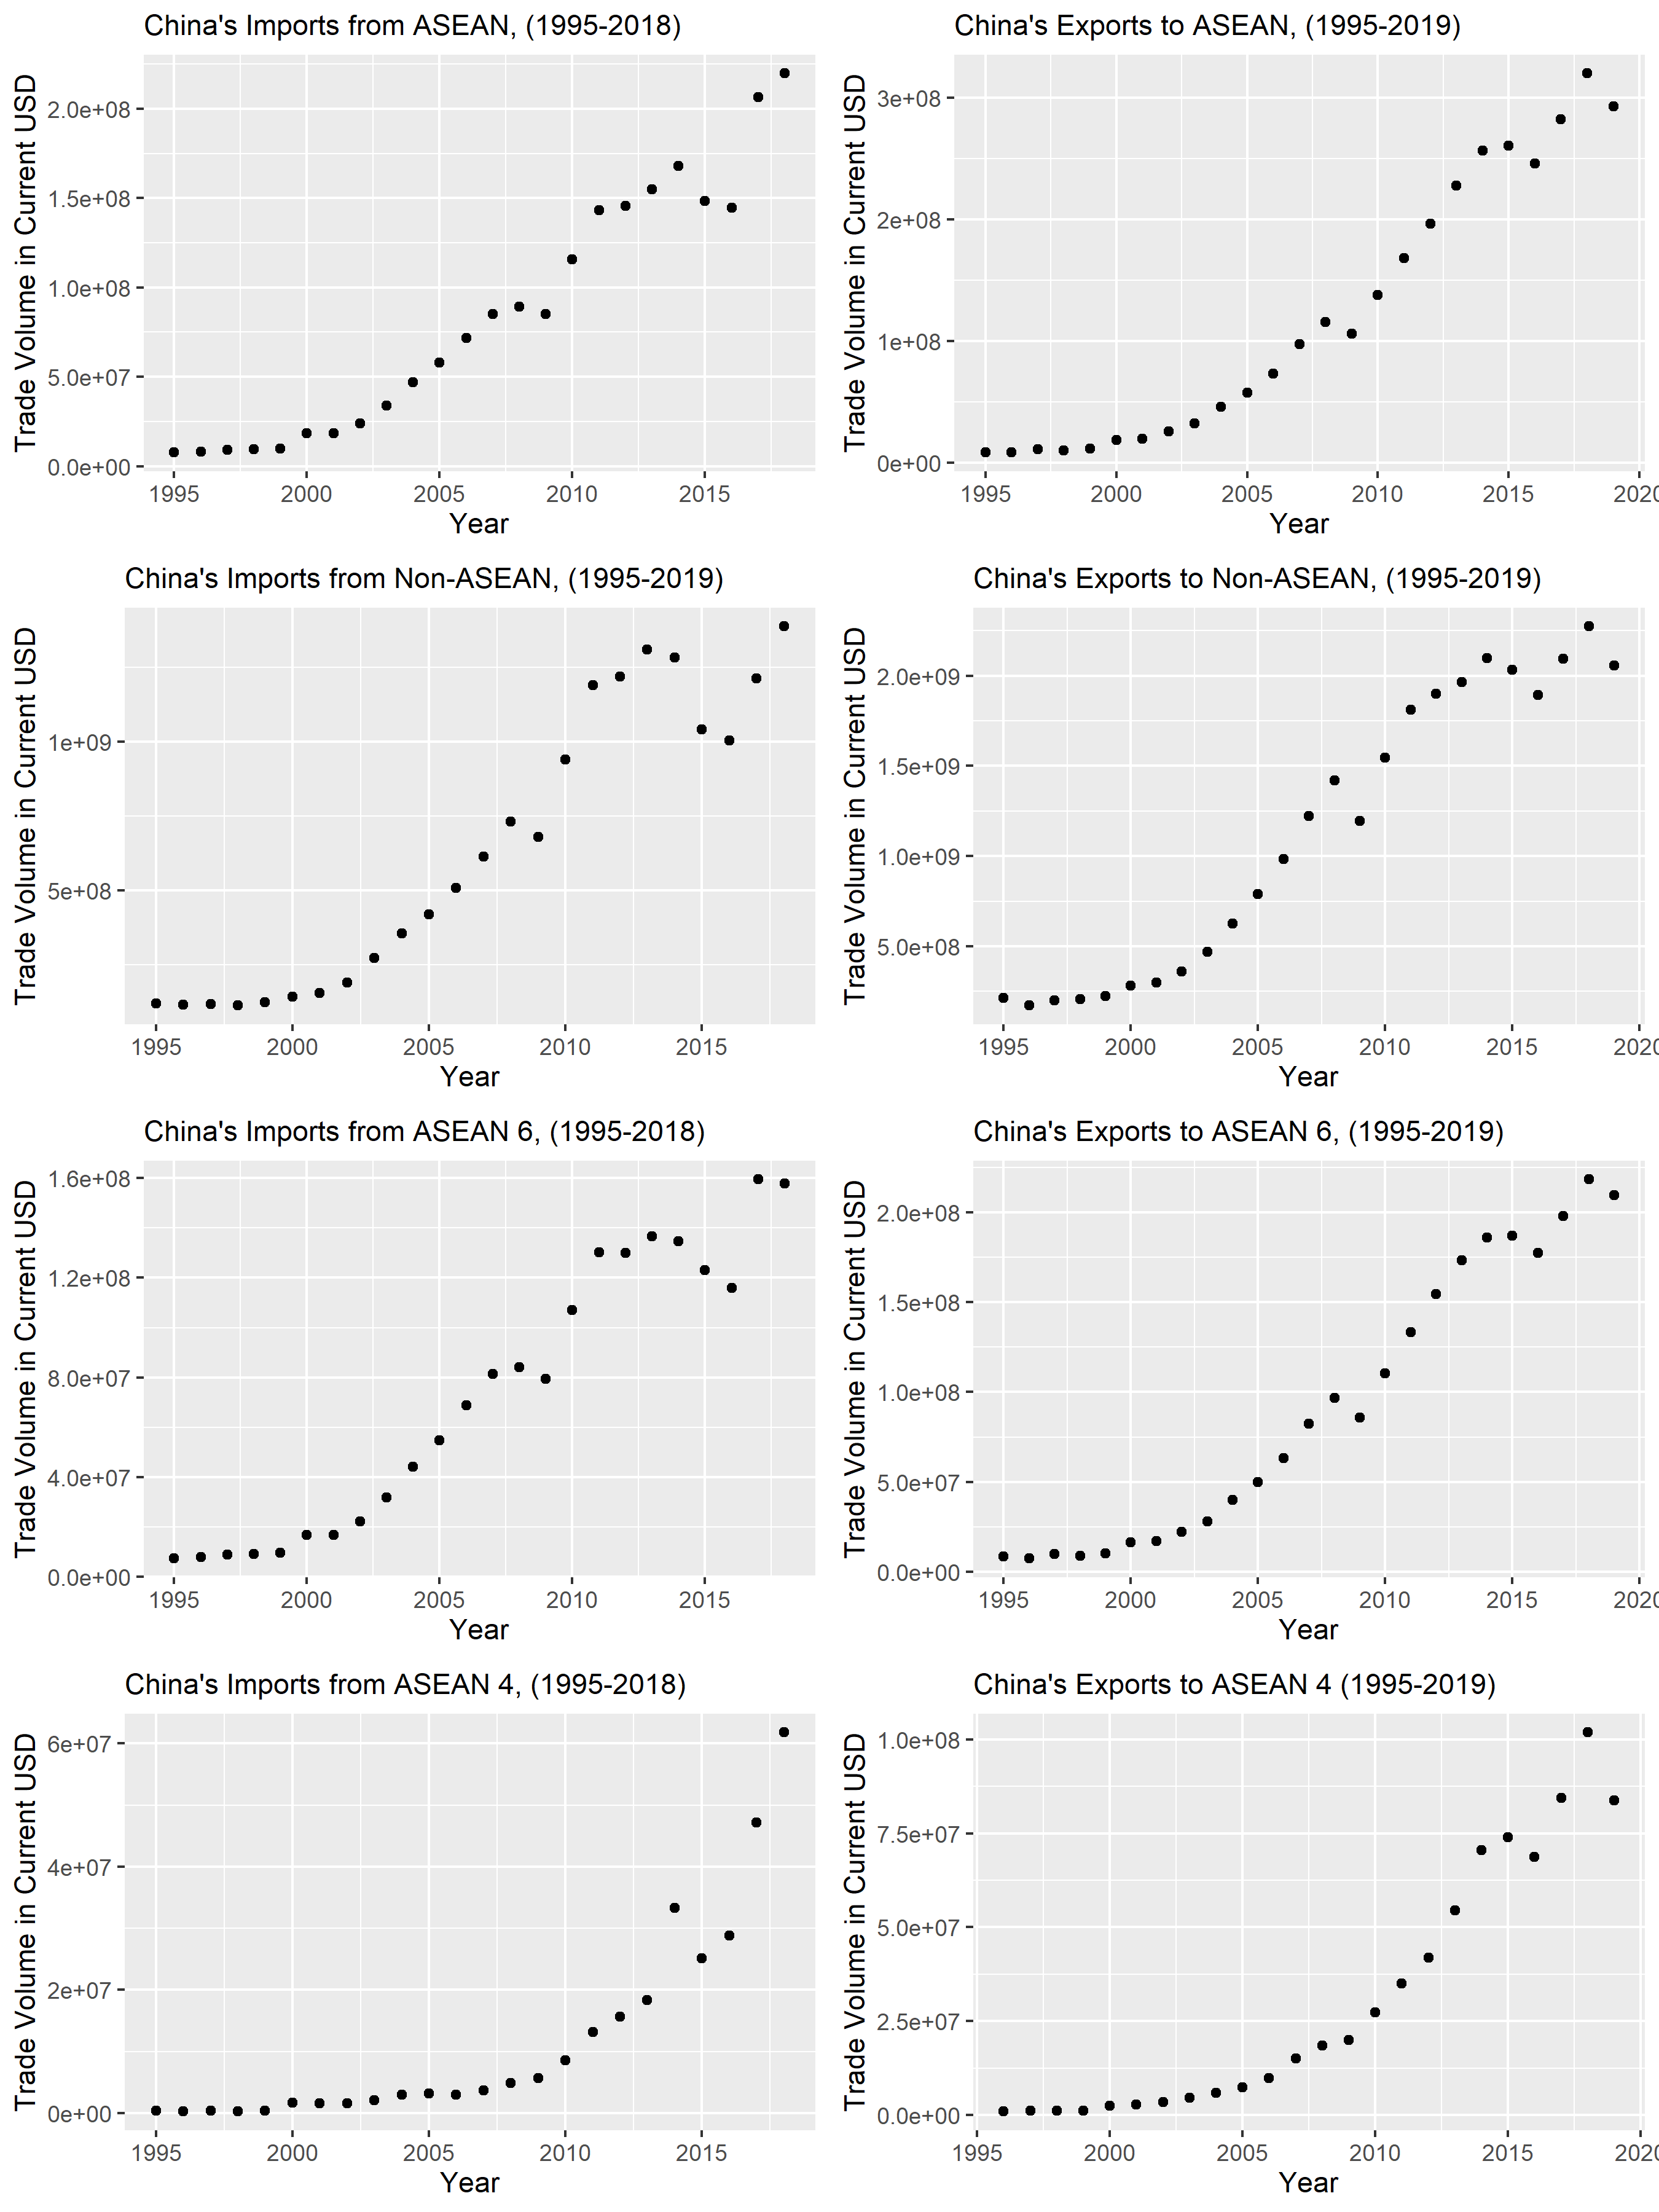
\includegraphics[height=18cm,width=\textwidth]{figure_1.png}
	\caption{\small{Evolution of Exports and Imports of ASEAN Countries with China over Time. Grouped by ASEAN6 and ASEAN4 Countries. \textit{Source:} UN Comtrade Import Data Retrieved in \cite{cepii-data_2022}.}}
	\label{fig_1}
\end{figure}

A potentially substantial part of the rise in trade flows can be associated with the tariff reduction and elimination program as described in Article 3 of the Agreement (\cite{asean_2002_1}). Article 3 foresees a gradual reduction in tariffs along two major categories. \footnote{See \cite{asean_2002_4}, as well as \cite{asean_2002_2} and \cite{asean_2002_3} for details.} \autoref{tab_1} shows that, depending on whether products were listed in the Normal or the Sensitive Track, applied MFN tariffs were to be reduced at different paces, between two different sets of countries. The first set of countries were the earlier ASEAN 6 member states Brunei, Indonesia, Malaysia, Philippines, Singapore and Thailand. The second set of countries were Cambodia, Lao, Myanmar and Vietnam ("ASEAN 4"). As seen, for ASEAN 6 and China, products listed in the Normal Track were to reduce or eliminate their respective applied MFN tariff rates gradually over a period from 1 January 2005 to 2010. In the case of the four newer ASEAN members, the period was from 1 January 2005 to 2015. ASEAN 6 and China were to reduce the applied MFN tariff rates of tariff lines placed in their respective Sensitive Track to 20\% not later than 1 January 2012. These tariff rates were then subsequently reduced to 0-5\% not later than 1 January 2018. Cambodia, Lao, Myanmar and Vietnam were to reduce the applied MFN tariff rates of tariff lines placed in their respective Sensitive Lists to 20\% not later than 1 January 2015. These tariff rates were then subsequently reduced to 0-5\% not later than 1 January 2020. 

\begin{table}[H]
\centering
\begin{tabular}{ccccc} 
\hline
\multicolumn{1}{l}{} & \multicolumn{1}{l}{}   & \textbf{Normal Track }                                                                                        & \multicolumn{2}{c}{\textbf{Sensitive Track}}                                                                                                \\ 
\cline{3-5}
\multicolumn{2}{c}{\textbf{Trade Partners}}   & \begin{tabular}[c]{@{}c@{}}\textbf{Applied MFN Tariff }\\\textbf{to be reduced}\\\textbf{until }\end{tabular} & \begin{tabular}[c]{@{}c@{}}\textbf{Applied MFN Tariff }\\\textbf{to be reduced }\\\textbf{to at least (\%)}\end{tabular} & \textbf{until }  \\ 
\hline
\textbf{ASEAN 6}     & \textbf{China}         & 1 January 2010                                                                                                & 20                                                                                                                       & 1 January 2012   \\
\textbf{ASEAN 6}     & \textbf{China}         & \multicolumn{1}{l}{}                                                                                          & 5                                                                                                                        & 1 January 2018   \\
\textbf{ASEAN 4}     & \textbf{China}         & 1 January 2015                                                                                                & 20                                                                                                                       & 1 January 2015   \\
\textbf{ASEAN 4}     & \textbf{China}         & \multicolumn{1}{l}{}                                                                                          & 5                                                                                                                        & 1 January 2020   \\
\hline
\end{tabular}
\caption{\small{ACFTA Tariff Liberalisation Along Two Different Country Groups and Products. \textit{Source:} \cite{asean_2002_1}.}}
\label{tab_1}
\end{table}

From the annexes of \cite{asean_2002_4} we infer that due to the vast heterogeneity of the tariff policy packages across countries, products and time, attributing trade flow effects to their respective tariff reduction episodes is beyond our scope. While this might sound discouraging at first, there is also another side of the medal. In addition to the tariff reductions, the Agreement foresees a row of further fields of economic integration (\cite{asean_2002_1}). For instance, the parties have agreed on gradually eliminating non-tariff barriers starting 1 January 2005. Furthermore, negotiators took into consideration the different stages of development among ASEAN member states: special conditions in connection to export facilitation were adopted in more recent member states such as Cambodia, Lao and Vietnam, in order for them to catch up in terms of domestic capacity, efficiency and competitiveness.

Given this heterogeneity in trade policies, our aim is to grasp the trade effects of the Agreement as a whole. In our gravity regressions, we account for this by using dummy variables that are meant to capture the entirety of trade liberalisation policies associated with ACFTA.

\end{subsection}

\begin{subsection}{Ex-Post Assessment of Regional Trade Agreements: The Gravity Model}

\begin{subsubsection}{Theoretical Foundation}
A common practice, we believe that starting with a gravity model is best to get an idea about the effects of a regional trade agreement. The structural gravity model describes how bilateral trade flows of country $i$ to country $j$ in period $t$ react to changes in the level of bilateral “freeness” of trade (\cite{mvzj_2019}). Thus, the main advantage of the structural gravity model is that it delivers a tractable framework for trade policy analysis in a multi-country environment. Following \cite{ypl_2016}, we motivate our choice by briefly explaining the structural gravity which our specifications rely upon. 

\begin{equation}\label{eq_1}
    Trade_{ij}=\frac{Y_{i}E_{j}}{Y}\Big(\frac{t_{ij}}{\Pi_{i}P_{j}}\Big)^{1-\sigma}
\end{equation}

The theoretical structural gravity equation \ref{eq_1} governs bilateral trade flows. It can be conveniently decomposed into two terms: (i) a size term $\frac{Y_{i}Y_{j}}{Y}$, (ii) and a trade cost term $\Big(\frac{t_{ij}}{\Pi_{i}P_{j}}\Big)^{1-\sigma}$.
\bigskip
\\
(i) The \textit{size term} consists of the world GDP ($Y$), the GDP of countries $i$ and $j$ ($Y_{i}$ and $Y_{j}$), respectively. Thus, it carries some very useful information regarding the relationship between country size and bilateral trade flows.
\bigskip
\\
(ii) The \textit{trade cost term} captures the total effects of trade costs that drive a wedge between realized and frictionless trade. The trade cost term consists of three components:
\begin{itemize}
\item Bilateral trade cost between partners $i$ and $j$, $t_{ij}$.
\item The structural term $P_{j}$ , coined by \cite{avw2003} as inward multilateral resistance represents importer $j$’s ease of market access.
\item The structural term $\Pi_{i}$, defined as outward multilateral resistance by \cite{avw2003}, measures exporter $i$’s ease of market access.
\end{itemize}

Given the multiplicative nature of the structural gravity equation \ref{eq_1}, and assuming that it holds in each period of time $t$, it is possible to log-linearize it and expand it with an additive error term:
\begin{equation}\label{eq_2}
   \ln{Trade_{ijt}}=\ln{Y_{jt}}+ \ln{Y_{it}}-\ln{Y_{t}}+(1-\sigma)\ln{t_{ijt}}-(1-\sigma)\ln{P_{jt}}-(1-\sigma)\ln{\Pi_{it}}+\varepsilon_{ijt}
\end{equation}
The standard practice suggested in the literature is to proxy for the
bilateral trade cost term, $(1-\sigma)\ln{t_{ijt}}$, by using a series of observable variables most of which have become standard covariates in empirical gravity specifications \cite{ypl_2016}:
\begin{equation}\label{eq_3}
(1-\sigma)\ln{t_{ijt}}=\beta_{1}\ln{Dist_{ij}} + \beta_2 Lang_{ij} + \beta_3 Contig_{ij} + \beta_4RTA_{ijt}+\varepsilon_{ijt}
\end{equation}

Inserting equation \ref{eq_3} into equation \ref{eq_2} yields the core idea behind our specifications. In order to obtain reliable estimates, we address several estimation techniques (see Section 3). 


\end{subsubsection}

\begin{subsubsection}{Empirical Review: Trade Creation, Trade Diversion or Both?}

\begin{figure}[H]
	\centering
	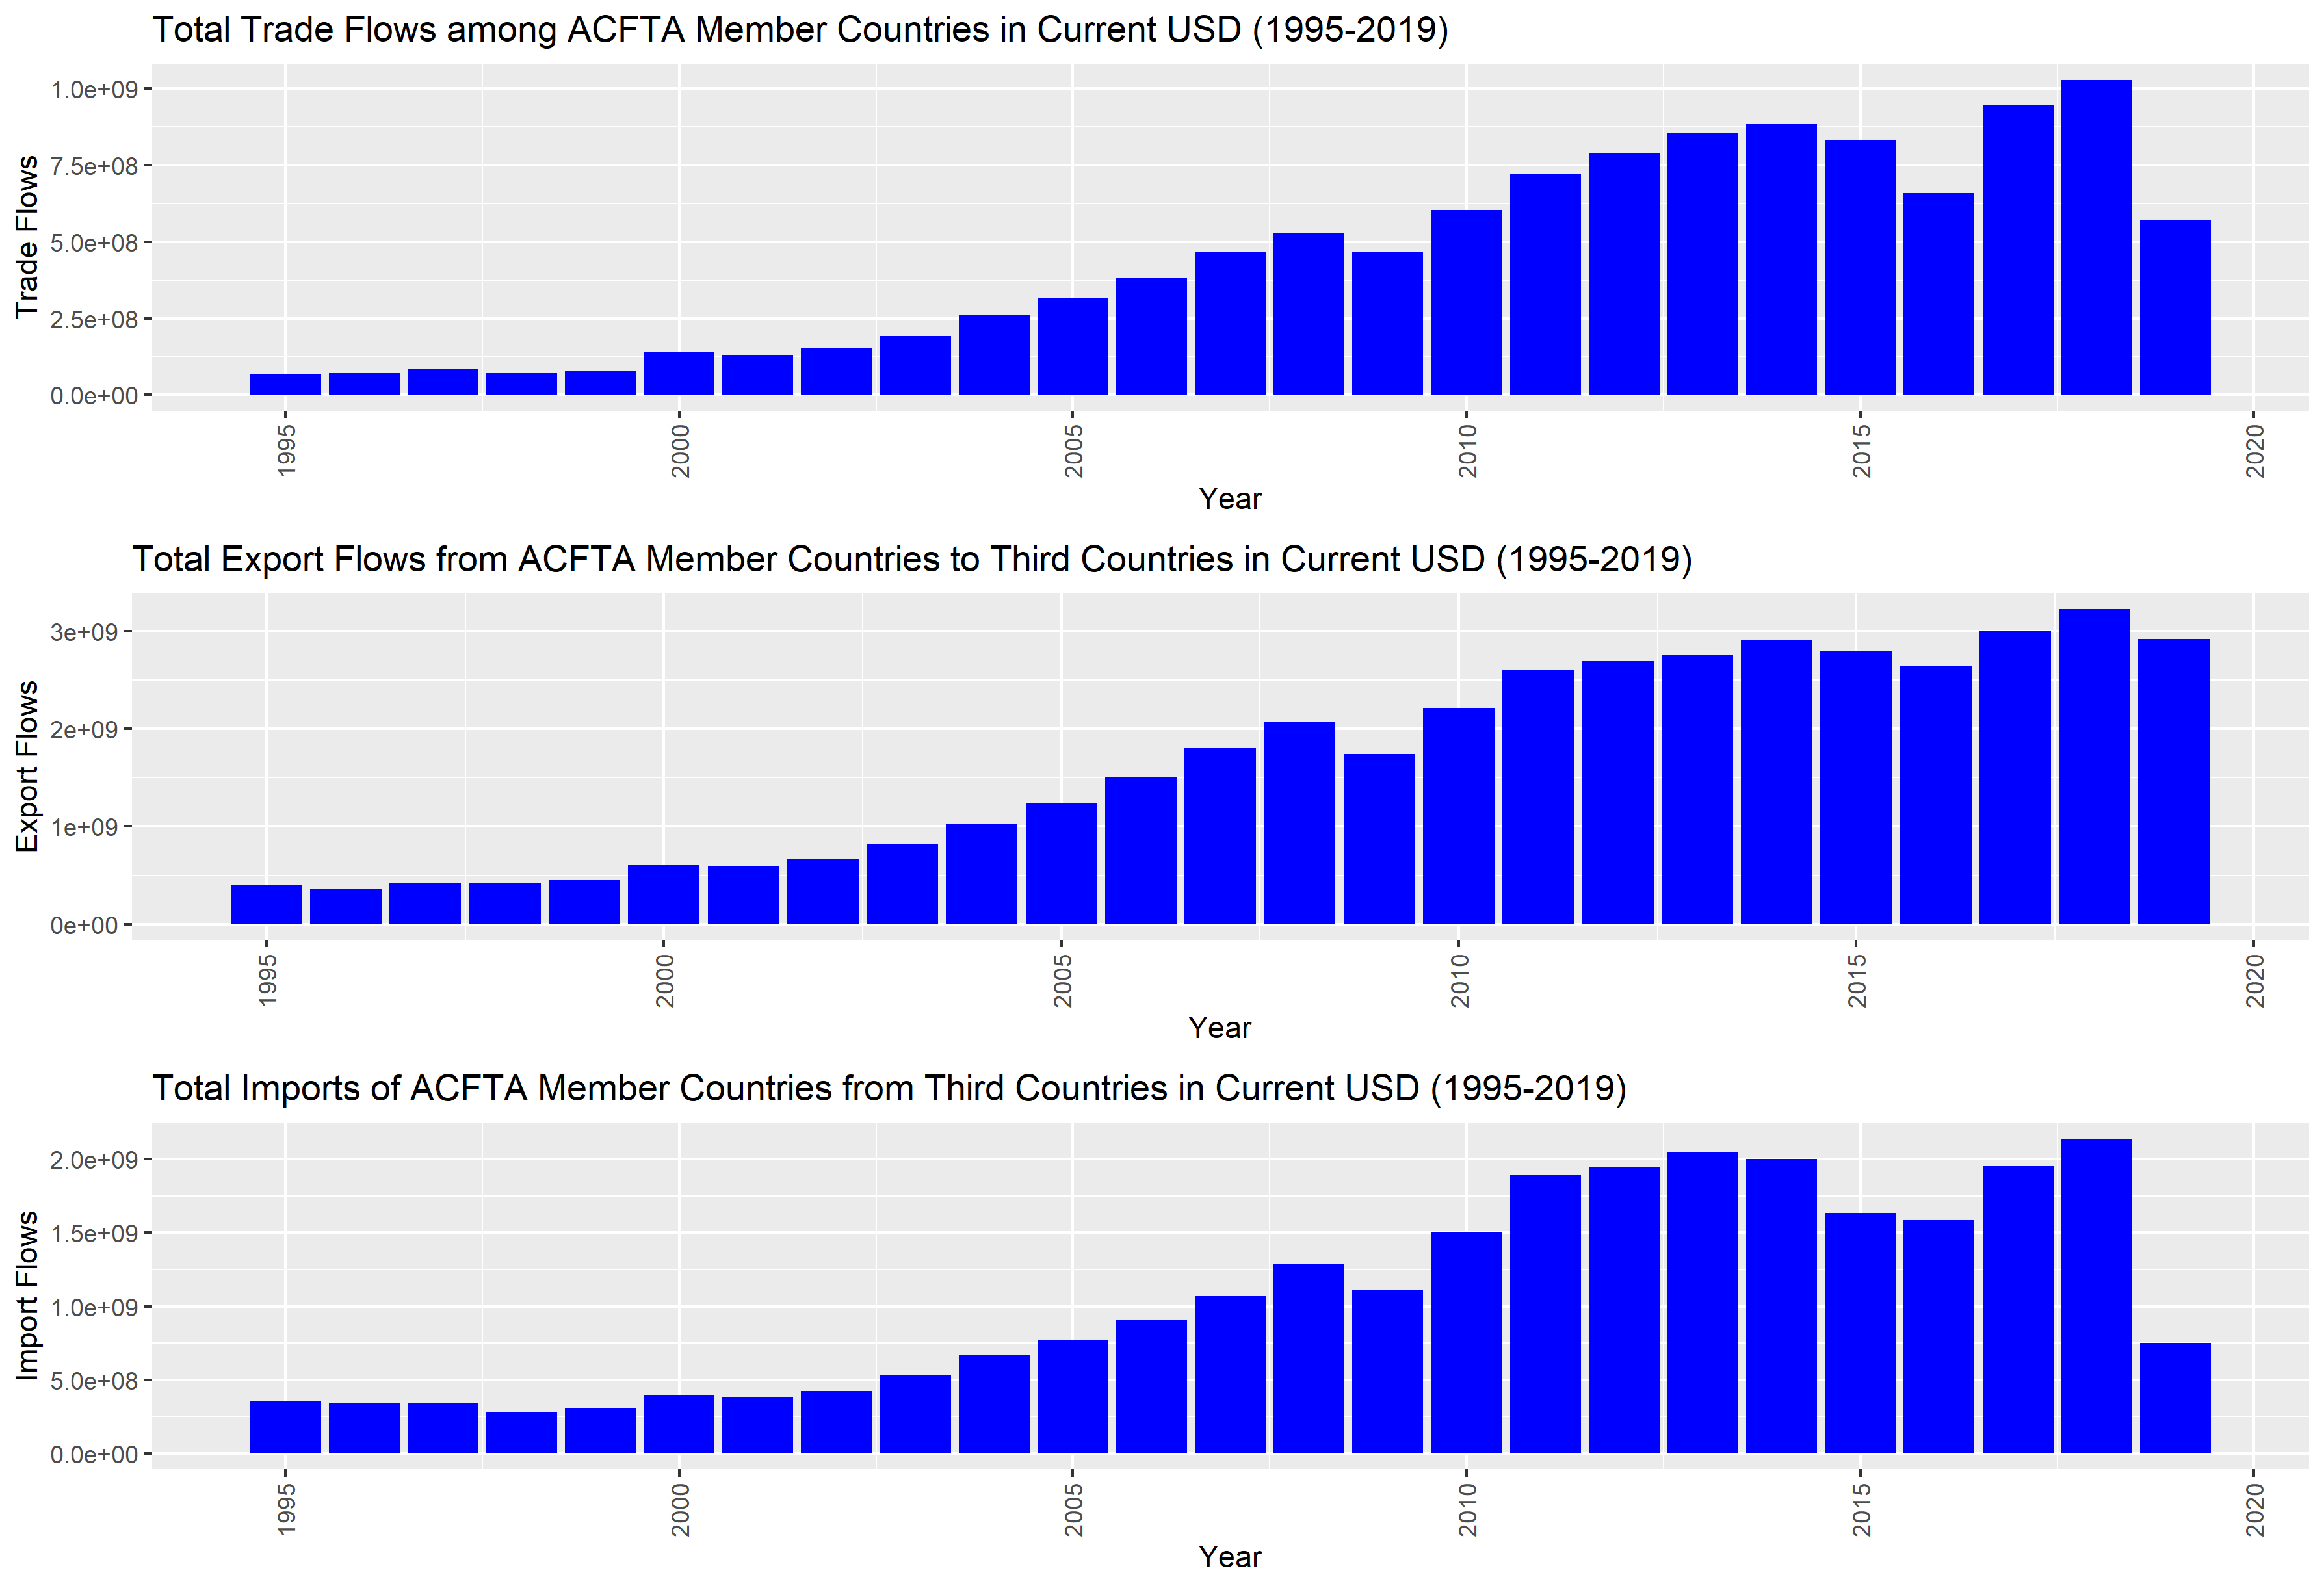
\includegraphics[width=\textwidth]{figure_2.png}
	\caption{\small{Trade Creation and Trade Diversion? Trade Flows Relating to ACFTA over Time. \textit{Source:} BACI Trade Flows Retrieved in \cite{cepii-data_2022}. Missing BACI Trade Flow Data were Replaced by UN Comtrade Import Data.}}
	\label{fig_2}
\end{figure}

This part intends to provide a brief survey of those papers closest to our methodology and regional trade integration episode. Conceptually, our aim to obtain trade integration effects goes back to \cite{viner1950}. Extending Viner's core idea of different trade effects, depending on whether a country is part of an integration episode or not, we model three different sets of FTA dummy variables representing trade creation and diversion effects in terms of export and import.\footnote{It was \cite{endoh1999} who first formalized this idea.} As our study intends to add to the grand debate around Vinerian trade creation and trade diversion in the literature on the ACFTA, we focus on studies that explore the trade impacts of ACFTA on ASEAN member countries, China and their respective third trading partners. 

\cite{smz2014}'s structural gravity framework intends to capture trade creation and trade diversion effects of ACFTA. They test their model on a sample of 31 countries over the period from 1995 to 2010 using UNCTAD export data for agricultural and manufactured goods and within manufactures for chemical products, as well as for machinery and transport equipment. Distinguishing between agricultural and manufacturing goods, they acknowledge the fact that the agreements involve different tariff-reduction schedules over time\footnote{Different provisions apply for agricultural goods (Early Harvest Products) and for manufacturing goods (Normal Track of the Agreement, see Section 2.1)}, and such can have distinctive effects on trade flows. Zooming in allows to examine sectors of particular importance for the overall trade effects.

A second study that uses a structural gravity framework is \cite{wla_2021}. The authors investigate the effects of exports from ACFTA to the 79 countries that together make up 95\% of ASEAN's export volume. In order to differentiate whether the formation of ACFTA has accelerated trade among both ASEAN member countries and non-ASEAN members, they employ three different dummy variables.  This allows them to separate between three different effects of trade creation and diversion, measured by export and import flows both within \textit{ACFTA} countries and between \textit{ACFTA} and \textit{Non-ACFTA} countries (see also \cite{carrere_2006}). First, the authors regress log trade flows on the dummies, controlling for GDP, population, language, distance and border contiguity, landlocked and islands in a pooled OLS regression. Second, they estimate the same specification with random effects. Finally, employing a battery of time-invariant fixed effects, the authors regress log trade flows on the dummies and log GDP and log population. 

Data on trade flows from the CEPII TradeProd and UN COMTRADE database of 2-digit ISIC manufacturing trade and FTAs for 64 countries during the period 1990–2002 at hand, \cite{dyz_2014} employ a structural gravity model to estimate effects of FTAs in terms of trade creation and trade diversion with a PPML estimator. 


\end{subsubsection}

\end{subsection}

\end{section}

\begin{section}{Methodology and Data }

\begin{subsection}{Methodology }

To answer our research question, our specifications need to allow for the possibility of trade creation and trade diversion.

\begin{figure}[H]
	\centering
	\includegraphics[width=\textwidth]{figure_4.png}
	\caption{\small{A Categorisation of Dummy Variables to Measure the Impact of Regional Trade Agreements.}}
	\label{fig_4}
\end{figure}

Our methodology departs from the $RTA$ dummy of \autoref{eq_4}. Our aim is to compare the effects of ACFTA on bilateral trade flows within ACFTA to ACFTA-sourced imports from third countries and ACFTA-directed exports from third countries. Therefore, we make use of three corresponding dummy variables as in \autoref{tab_2}. It is this triad of dummy variables that enables us to obtain evidence on the so-called Viner ambiguity in the context of the ACFTA (see \autoref{tab_2}). Our study is to be viewed as adding robustness to \cite{smz2014} and \cite{wla_2021}. Furthermore, we include a dummy that captures trade flows occurring between all other third countries that are part of an RTA that is different from ACFTA. This helps us to compare the strength of the ACFTA RTA to the strength of all other RTAs in the world. In our specifications, their combined effect is captured by the \textbf{$otherRTA$} dummy.

\textbf{\textbf{$ACFTA_{intra}$}} estimates the impact of the commencement of the agreement on ASEAN-China trade flows. Throughout all specifications, $ACFTA$ takes the value one when countries $i$ and $j$ belong to ACFTA in year $t$ and zero if otherwise. A positive (negative) coefficient $\gamma_1$ represents trade creation (diversion), depending on whether intra-bloc trade is higher (lower) than the normal trade levels due to the trade agreement. 

\textbf{\textbf{$ACFTA_{export}$} }takes a value of one if exporter country $i$ belongs to the ACFTA in year $t$ and destination country $j$ does not belong to the ACFTA countries and zero otherwise. A statistically significant and positive $\delta_1$ coefficient can be interpreted as an export creation effect. It implies that regional trade integration leads to export diversion from ACFTA member countries to non-ACFTA countries. However, a negative $\delta_1$ coefficient signifies an export reduction between member countries and non-member countries, known as the export diversion effect (\cite{carrere_2006}). 

\textbf{\textbf{$ACFTA_{import}$}} takes a value of one if exporter $i$ is a non-member country of ACFTA in year $t$ and destination country $j$ belongs to the ACFTA member countries and zero otherwise. Essentially, a statistically significant and positive $\delta_2$ coefficient captures an import creation effect, showing the expansion of imports from the non-member countries to member countries. Contrarily, a negative $\delta_2$ coefficient indicates the import diversion effect, a decrease in imports from non-member- to member countries (\cite{carrere_2006}).

Our ex-post assessment of the trade effects of ACFTA starts with a naïve regression specification, and considers only international trade flows (i.e. for $i \neq j$). Stepwise, we include additional modifications. Each modification introduces a new feature to the initial specification, aiming at correctly identified estimates of the three ACFTA effects and the RTA-comparison.

\subsubsection*{Specification 1: OLS estimation ignoring multilateral resistance terms}

We first do an OLS estimation of the empirical specification that includes standard gravity variables with panel data with 4-year intervals\footnote{Interval panel data should be employed in order to allow for adjustment in bilateral trade flows in response to trade policy or other changes in trade costs (\cite{ypl_2016})}:

\begin{multline}\label{eq_5}
\ln{Trade_{ijt}} = \alpha_0 + \beta_1 \ln{Y_{it}} + \beta_2 \ln{Y_{jt}} + \beta_3 \ln{Pop_{it}} + \beta_4 \ln{Pop_{jt}}  + \beta_5 \ln{Dist_{ij}} + \beta_6 Lang_{ij} + \beta_7 Contig_{ij} + \\
\gamma_1 ACFTAintra_{ijt} + \gamma_2 otherRTA_{ijt} + \\ 
\delta_1 ACFTAexport_{ijt} + \delta_2 ACFTAimport_{ijt} + \epsilon_{ijt}
\end{multline}

In this basic gravity model, we make aggregate total bilateral trade flows $lnTrade$ from to country $j$ to country $i$ dependent on Gross Domestic Product ($lnY$), population ($lnPop$) and distance ($lnDist$). Moreover, we include the binary dummies common border ($Contig$) and language ($Lang$). 


\subsubsection*{Specification 2: OLS estimation controlling for multilateral resistance terms with fixed effects}

As the theoretical foundation, the multilateral resistance terms $P_{j,t}$ and $Pi_{i,t}$ should be properly controlled in the gravity model; however, the difficulty is that they are not directly observable by the researcher and/or by the policymaker. \cite{Feenstra2016} proposes and demonstrates that multilateral resistance terms should be accounted for by exporter-time and importer-time fixed effects in a dynamic gravity estimation framework with panel data to overcome this challenge. In this way, the exporter-time and importer-time fixed effects will also absorb the size variables ($E_{j,t}$ and $Y_{i,t}$ ) from the structural gravity model as well as all other observable and unobservable country-specific characteristics.

Thus, specification \ref{eq_5} is modified to account for the multilateral resistances as follows.

\begin{multline}\label{eq_6}
\ln{Trade_{ijt}} = \mu_{it} + \phi_{jt} + \beta_5 \ln{Dist_{ij}} + \beta_6 Lang_{ij} + \beta_7 Contig_{ij} + \\ \gamma_1 ACFTAintra_{ijt} + \gamma_2 otherRTA_{ijt} +  \epsilon_{ijt}
\end{multline}

$\mu_{it}$ denotes the vector of exporter-time fixed effects, which accounts for the outward multilateral resistances. Similarly, the vector $\phi_{jt}$ denotes the set of importer-time fixed effects to capture the inward multilateral resistances. No constant term is included in the presence of the fixed effects.


\subsubsection*{Specification 3: PPML estimation controlling for multilateral resistance terms with fixed effects}

Specification \ref{eq_6} is re-formulated in multiplicative form and re-estimated by applying the PPML estimator to the same sample (with international trade only).

\begin{multline}\label{eq_7}
Trade_{ijt} = exp \Big(\mu_{it} + \phi_{jt} + \beta_5 lnDist_{ij} + \beta_6 Lang_{ij} + \beta_7 Contig_{ij} \\ 
+ \gamma_1 ACFTAintra_{ijt} + \gamma_2 otherRTA_{ijt} \Big) \epsilon_{ijt}
\end{multline}

\bigskip
Applying the PPML estimator to the gravity model is justified on various grounds. First, the PPML estimator expressed in a multiplicative form, accounts for heteroscedasticity, which often plagues trade data (\cite{silva2006log}). Second, for the same reason, the PPML estimator is able to take advantage of the information contained in the zero trade flows. Third, the additive property of the PPML estimator ensures that the gravity fixed effects are identical to their corresponding structural terms (\cite{fally2015}).

\subsubsection*{Specification 4: Addressing potential endogeneity of FTAs}

Without further ado, trade effects from the formation of ACFTA could have lied fault to a chicken egg problem of reverse causality. Following \cite{ypl_2016}, specification \ref{eq_7} is modified to include country-pair fixed effects $\pi_{ij}$ in addition to the importer-time and exporter-time fixed effects $\mu_{it}$ and $\phi_{jt}$.

\begin{multline}\label{eq_8}
Trade_{ijt} = exp \Big(\mu_{it} + \phi_{jt} + \pi_{ij} + 
\gamma_1 ACFTA_{ijt} + \gamma_2 otherRTA_{ijt}\Big) \epsilon_{ijt}
\end{multline}

Our rationale stems from \cite{bb_2007} who warn of omitted variable bias and simultaneity bias. 
To illustrate a potential source of omitted variable bias, let us suppose two countries with extensive domestic regulations inhibiting trade. Then, once a large expected welfare gain from trade creation via the FTA in sight, the likelihood of the countries selecting into the FTA could have been especially high. 
Simultaneity bias can be illustrated as follows: suppose two countries trade more or less than the gravity-equation-suggested “natural” level. This could be due to an already extensive trading relationship. Contrarily, one can imagine political pressures to avoid trade liberalisation. In both cases, the problem is that the decision to form an FTA is likely influenced by trade relative to the “natural” level. In contrast, recent changes in trade levels are unlikely to influence FTA formations. Hence, looking at recent changes in trade levels between country pairs allows control for the “natural” level of trade. The idea is that unobserved time invariant heterogeneity, hidden in the “natural” level of trade, simultaneously influences the presence of a FTA and the volume of trade. Using panel data we can control for this unobserved time invariant heterogeneity. Exploiting cross-sectional unit variation over time, we can be reassured about identification. 

\end{subsection}



\begin{subsection}{Data}

This study uses unbalanced panel data of bilateral trade flows, GDP, population, distance, geographical, cultural and historical information and a few other group-specific measures from \cite{cepii-data_2022}.

The gravity models include 252 countries covering the period 1995-2019 (24 years). The source of information for aggregated (country-level) bilateral trade flows is BACI trade data downloaded from \cite{cepii-data_2022}. The reason for choosing BACI data for the dependent variable is twofold: first, BACI data are cleaned to exclude re-exports and re-imports. Second, BACI data reconcile reporting differences among countries \cite{gaulier2010baci}. Therefore, BACI data provide a more complete and coherent set of trade flows. We however stick to UN Comtrade import data to replace missing values of BACI trade flows. Again, there are two reasons. First, BACI trade flows stem from the UN Comtrade database. Second, import data is considered more reliable because imports are monitored much more closely than exports by customs administrations, see \cite{ypl_2016}.

Please, find the code and data for reproduction \href{https://github.com/gerodasbach/data_repository_RIA_report.git}{here}.\footnote{Due to the large size of the original data set, it is not part of the github repository. We offer to transfer it and suggest to insert it manually into your \textit{./input} folder. Please contact us per \href{mailto:gero.dasbach@gmail.com}{e-mail}.}

\end{subsection}
\end{section}


\begin{section}{Results}
\autoref{tab_3} shows our results.

\textbf{Specification 1.}
At a high explanatory power ($R^2 = 64\%$), all standard gravity variables except population are statistically significant and resemble the expected signs. We find that the impact of population on bilateral trade is positive for importers and negative for exporters. According to \cite{wla_2021}, this could be due to firstly, larger exporter populations implying larger domestic markets, richer resource endowment and more diversified outputs, as well as less dependence on international specialisation. Secondly, a larger population in an importing country could enhance competition between imported and domestic goods and compensate exporters for the cost of sales activities abroad.

We obtain high average treatment effects of trade relative to the "normal" level. The coefficient $\gamma_1$ shows an increase of trade within the ACFTA of $(e^{1.326}-1)=276\%$. The increase in exports between ACFTA countries and third countries relative to the natural level is ($\delta_1$) 199\%. Imports between ACFTA countries and third countries ($\delta_2$) increase by 31\%. Thus, this model confirms our hypothesis of pure trade creation (compare \autoref{fig_2}). Furthermore, trade flows between ACFTA and third-country partners in another FTA ($otherRTA$) increase by 109\%.

Contrary to our OLS results, \cite{wla_2021}'s pooled OLS coefficients for $\gamma_1$, $\delta_1$ and $\delta_2$ are of the other sign. However, their fixed effects model results show positive signs for all three coefficients. The magnitude of the increase in trade flows (228\%, 272\% and 147\%) they obtain with OLS fixed effects differs only slightly from our OLS results for $\gamma_1$, $\delta_1$ and $\delta_2$. \cite{wla_2021} explain their confirmation of the pattern of pure trade creation (see \autoref{fig_2}) with the expansion of global value chains in the ASEAN region. They claim that intra-industry trade within ACFTA has generated significant momentum for world trade overall. Furthermore, they point out the development and harmonization of product standards as crucial for trade-enhancement in the context of regional trade agreements.

\textbf{Specification 2.}
The benefit from multilateral resistance terms is that we can put trade barriers within ACFTA into perspective to average trade barriers that ACFTA faces with all of their other FTA trading partners. Comparing $\gamma_1$ and the coefficient of $otherRTA$ to the results of specification 1 allows us to obtain an idea about the importance of multilateral resistance in numbers. Indeed, at high explanatory power ($R^2 = 74\%$) we obtain different results. While $\gamma_1$ becomes statistically insignificant, the $otherRTA$ effect remains significant and positive (+75\%).  

\textbf{Specification 3.}
Using a PPML estimator as in \cite{dyz_2014}, we do not obtain statistically significant results on intra-ACFTA trade flows. The coefficient of $otherRTA$ becomes slightly smaller than in the OLS fixed effects estimation of specification 2 (+48\%). A comparison to \cite{dyz_2014}'s results shows: although very similar in methodology to \cite{dyz_2014}, our study rejects their hypothesis that an FTA leads to trade diversion in the case of the ACFTA. We obtain this result by comparing the sign of our dummy $otherRTA$ to the combined effect of their "Outside FTA (imp)" and "Outside FTA (exp)" dummies.

\textbf{Specification 4.}
\autoref{fig_3} illustrates the concept behind our results for specification 4. Although clearly not a highly significant decrease of -57\% for the average importer country sharing an FTA with a given FTA member country (\cite{dyz_2014}), we find that the magnitude of trade creation within ACFTA and between ACFTA and its third-FTA trade partners is different at the 90\% confidence level. While the ACFTA bloc witnesses an increase in trade flows by 31\%, trade with ACFTA's third FTA partner countries increases by 8\%.  

Unfortunately, our $ACFTAexport$ and $ACFTAimport$ dummies get dropped because of multicollinearity. We still want to mention results of the literature.\footnote{\cite{smz2014}'s $ACFTAexport$ and $ACFTAimport$ dummies do not get dropped due to multicollinearity.} Positive and more significant, \cite{smz2014}'s country-pair fixed effects coefficient $\gamma_1$ shows an increase in trade higher than ours (119\% vs. 31\%). 

In line with our results from specification 1, the authors find evidence for unambiguous trade creation across all three dummies: while exports to non-ACFTA countries rise by 58\%, imports from non-ACFTA countries to the bloc increase by 40\%. Using the PML method, their results for the agricultural and manufacturing sector are able to capture zero trade flows and large levels of heteroscedasticity, well. Their results for trade creation are confirmed for trade within ACFTA and exports from ACFTA for manufactured goods and within manufactures for chemical products, as well as for machinery and transport equipment. Only for imports from countries not part of the ACFTA they find effects of trade diversion. Net trade creation is $130\%$ for manufactured goods, $120\%$ for chemical goods and $36\%$ for machinery and transport equipment. This order of magnitudes in their effects resembles the order of magnitude of our obtained estimates of specification 1. Due to the difficulties of interpreting the magnitude of our naive gravity OLS estimates, we cannot assess the claim of \cite{wla_2021} whether it is plausible that it was intra-industry trade within ACFTA that has boosted the pure trade creation effects they obtain.

\end{section}

\begin{section}{Conclusion}

We cannot reject our first hypothesis of pure trade creation. However, we have to acknowledge that our results are based upon a naive OLS gravity regression. Comparing our results to the literature, we find that our claim is backed up by other studies examining the ACFTA, in particular, for slightly different time frames and data on specific sectors. Although our results resemble the pattern of a sustained increase in trade flows as in \autoref{fig_2}, we lack an econometrically sound approach to evaluate them. A solution could lie in including internal trade flows to avoid collinearity in $ACFTAexport$ and $ACFTAimport$ dummies with country-time FE, although obtaining consistently measured internal trade is challenging.

We cannot reject our second hypothesis that the ACFTA yields more trade creation than all other FTAs excluding ACFTA countries. Consulting the literature, and \cite{wla_2021} in particular, we hold it probable that the embeddedness of ACFTA countries in global supply chains is an explanatory factor behind ACFTA not leading to external trade diversion. The limited econometric power of our naive gravity model results makes it impossible to evaluate this claim. 

The average efficiency of the ACFTA in terms of trade volume effect is relatively higher than that of the rest of the world's RTAs. Moreover, we find that when taking China out, trade was increasing through FTAs in other parts of the world, as well. Ratified just three years after China's WTO accession in 2001, it is likely that dummy variables on trade diversion (e.g. as in \cite{dyz_2014}) are biased by this crucial step of China's global trade integration. The good news is that our dummy allows us to split within-ACFTA effects from other RTA effects that do not contain China.

Moreover, in feedback with our literature, we take away that trade creation in ACFTA is most pronounced within the bloc, followed by exports from ACFTA. There is less safe evidence for imports from countries outside the ACFTA.

\end{section}



  \providecommand{\huxb}[2]{\arrayrulecolor[RGB]{#1}\global\arrayrulewidth=#2pt}
  \providecommand{\huxvb}[2]{\color[RGB]{#1}\vrule width #2pt}
  \providecommand{\huxtpad}[1]{\rule{0pt}{#1}}
  \providecommand{\huxbpad}[1]{\rule[-#1]{0pt}{#1}}

\begin{table}[ht]
\begin{centerbox}
\begin{threeparttable}
\captionsetup{justification=centering,singlelinecheck=off}
\caption{Estimating the Effects of the ASEAN-China Free Trade Agreement}
 \label{tab_3}
\setlength{\tabcolsep}{0pt}
\begin{tabularx}{1\textwidth}{p{0.3\textwidth} p{0.175\textwidth} p{0.175\textwidth} p{0.175\textwidth} p{0.175\textwidth}}


\hhline{>{\huxb{0, 0, 0}{1}}->{\huxb{0, 0, 0}{1}}->{\huxb{0, 0, 0}{1}}->{\huxb{0, 0, 0}{1}}->{\huxb{0, 0, 0}{1}}-}
\arrayrulecolor{black}

\multicolumn{1}{!{\huxvb{0, 0, 0}{0}}p{0.3\textwidth}!{\huxvb{0, 0, 0}{0}}}{\hspace{6pt}\parbox[b]{0.3\textwidth-6pt-6pt}{\huxtpad{0pt + 1em}\centering \huxbpad{0pt}}} &
\multicolumn{1}{p{0.175\textwidth}!{\huxvb{0, 0, 0}{0}}}{\hspace{6pt}\parbox[b]{0.175\textwidth-6pt-6pt}{\huxtpad{0pt + 1em}\centering (1) OLS\huxbpad{0pt}}} &
\multicolumn{1}{p{0.175\textwidth}!{\huxvb{0, 0, 0}{0}}}{\hspace{6pt}\parbox[b]{0.175\textwidth-6pt-6pt}{\huxtpad{0pt + 1em}\centering (2) OLS\huxbpad{0pt}}} &
\multicolumn{1}{p{0.175\textwidth}!{\huxvb{0, 0, 0}{0}}}{\hspace{6pt}\parbox[b]{0.175\textwidth-6pt-6pt}{\huxtpad{0pt + 1em}\centering (3) PPML\huxbpad{0pt}}} &
\multicolumn{1}{p{0.175\textwidth}!{\huxvb{0, 0, 0}{0}}}{\hspace{6pt}\parbox[b]{0.175\textwidth-6pt-6pt}{\huxtpad{0pt + 1em}\centering  (4) ENDG\huxbpad{0pt}}} \tabularnewline[-0.5pt]


\hhline{}
\arrayrulecolor{black}

\multicolumn{1}{!{\huxvb{0, 0, 0}{0}}p{0.3\textwidth}!{\huxvb{0, 0, 0}{0}}}{\hspace{6pt}\parbox[b]{0.3\textwidth-6pt-6pt}{\huxtpad{0pt + 1em}\centering \huxbpad{0pt}}} &
\multicolumn{1}{p{0.175\textwidth}!{\huxvb{0, 0, 0}{0}}}{\hspace{6pt}\parbox[b]{0.175\textwidth-6pt-6pt}{\huxtpad{0pt + 1em}\centering  \huxbpad{0pt}}} &
\multicolumn{1}{p{0.175\textwidth}!{\huxvb{0, 0, 0}{0}}}{\hspace{6pt}\parbox[b]{0.175\textwidth-6pt-6pt}{\huxtpad{0pt + 1em}\centering Fixed Effects\huxbpad{0pt}}} &
\multicolumn{1}{p{0.175\textwidth}!{\huxvb{0, 0, 0}{0}}}{\hspace{6pt}\parbox[b]{0.175\textwidth-6pt-6pt}{\huxtpad{0pt + 1em}\centering Fixed Effects\huxbpad{0pt}}} &
\multicolumn{1}{p{0.175\textwidth}!{\huxvb{0, 0, 0}{0}}}{\hspace{6pt}\parbox[b]{0.175\textwidth-6pt-6pt}{\huxtpad{0pt + 1em}\centering Fixed Effects\huxbpad{0pt}}} \tabularnewline[-0.5pt]


\hhline{>{\huxb{255, 255, 255}{0.4}}->{\huxb{0, 0, 0}{0.4}}->{\huxb{0, 0, 0}{0.4}}->{\huxb{0, 0, 0}{0.4}}->{\huxb{0, 0, 0}{0.4}}-}
\arrayrulecolor{black}

\multicolumn{1}{!{\huxvb{0, 0, 0}{0}}p{0.3\textwidth}!{\huxvb{0, 0, 0}{0}}}{\hspace{6pt}\parbox[b]{0.3\textwidth-6pt-6pt}{\huxtpad{0pt + 1em}\raggedright log exporter's GDP\huxbpad{0pt}}} &
\multicolumn{1}{p{0.175\textwidth}!{\huxvb{0, 0, 0}{0}}}{\hspace{6pt}\parbox[b]{0.175\textwidth-6pt-6pt}{\huxtpad{0pt + 1em}\centering 1.182 ***\huxbpad{0pt}}} &
\multicolumn{1}{p{0.175\textwidth}!{\huxvb{0, 0, 0}{0}}}{\hspace{6pt}\parbox[b]{0.175\textwidth-6pt-6pt}{\huxtpad{0pt + 1em}\centering \huxbpad{0pt}}} &
\multicolumn{1}{p{0.175\textwidth}!{\huxvb{0, 0, 0}{0}}}{\hspace{6pt}\parbox[b]{0.175\textwidth-6pt-6pt}{\huxtpad{0pt + 1em}\centering \huxbpad{0pt}}} &
\multicolumn{1}{p{0.175\textwidth}!{\huxvb{0, 0, 0}{0}}}{\hspace{6pt}\parbox[b]{0.175\textwidth-6pt-6pt}{\huxtpad{0pt + 1em}\centering \huxbpad{0pt}}} \tabularnewline[-0.5pt]


\hhline{}
\arrayrulecolor{black}

\multicolumn{1}{!{\huxvb{0, 0, 0}{0}}p{0.3\textwidth}!{\huxvb{0, 0, 0}{0}}}{\hspace{6pt}\parbox[b]{0.3\textwidth-6pt-6pt}{\huxtpad{0pt + 1em}\raggedright \huxbpad{0pt}}} &
\multicolumn{1}{p{0.175\textwidth}!{\huxvb{0, 0, 0}{0}}}{\hspace{6pt}\parbox[b]{0.175\textwidth-6pt-6pt}{\huxtpad{0pt + 1em}\centering (0.007)\huxbpad{0pt}}} &
\multicolumn{1}{p{0.175\textwidth}!{\huxvb{0, 0, 0}{0}}}{\hspace{6pt}\parbox[b]{0.175\textwidth-6pt-6pt}{\huxtpad{0pt + 1em}\centering \huxbpad{0pt}}} &
\multicolumn{1}{p{0.175\textwidth}!{\huxvb{0, 0, 0}{0}}}{\hspace{6pt}\parbox[b]{0.175\textwidth-6pt-6pt}{\huxtpad{0pt + 1em}\centering \huxbpad{0pt}}} &
\multicolumn{1}{p{0.175\textwidth}!{\huxvb{0, 0, 0}{0}}}{\hspace{6pt}\parbox[b]{0.175\textwidth-6pt-6pt}{\huxtpad{0pt + 1em}\centering \huxbpad{0pt}}} \tabularnewline[-0.5pt]


\hhline{}
\arrayrulecolor{black}

\multicolumn{1}{!{\huxvb{0, 0, 0}{0}}p{0.3\textwidth}!{\huxvb{0, 0, 0}{0}}}{\hspace{6pt}\parbox[b]{0.3\textwidth-6pt-6pt}{\huxtpad{0pt + 1em}\raggedright log importer's GDP\huxbpad{0pt}}} &
\multicolumn{1}{p{0.175\textwidth}!{\huxvb{0, 0, 0}{0}}}{\hspace{6pt}\parbox[b]{0.175\textwidth-6pt-6pt}{\huxtpad{0pt + 1em}\centering 0.830 ***\huxbpad{0pt}}} &
\multicolumn{1}{p{0.175\textwidth}!{\huxvb{0, 0, 0}{0}}}{\hspace{6pt}\parbox[b]{0.175\textwidth-6pt-6pt}{\huxtpad{0pt + 1em}\centering \huxbpad{0pt}}} &
\multicolumn{1}{p{0.175\textwidth}!{\huxvb{0, 0, 0}{0}}}{\hspace{6pt}\parbox[b]{0.175\textwidth-6pt-6pt}{\huxtpad{0pt + 1em}\centering \huxbpad{0pt}}} &
\multicolumn{1}{p{0.175\textwidth}!{\huxvb{0, 0, 0}{0}}}{\hspace{6pt}\parbox[b]{0.175\textwidth-6pt-6pt}{\huxtpad{0pt + 1em}\centering \huxbpad{0pt}}} \tabularnewline[-0.5pt]


\hhline{}
\arrayrulecolor{black}

\multicolumn{1}{!{\huxvb{0, 0, 0}{0}}p{0.3\textwidth}!{\huxvb{0, 0, 0}{0}}}{\hspace{6pt}\parbox[b]{0.3\textwidth-6pt-6pt}{\huxtpad{0pt + 1em}\raggedright \huxbpad{0pt}}} &
\multicolumn{1}{p{0.175\textwidth}!{\huxvb{0, 0, 0}{0}}}{\hspace{6pt}\parbox[b]{0.175\textwidth-6pt-6pt}{\huxtpad{0pt + 1em}\centering (0.007)\huxbpad{0pt}}} &
\multicolumn{1}{p{0.175\textwidth}!{\huxvb{0, 0, 0}{0}}}{\hspace{6pt}\parbox[b]{0.175\textwidth-6pt-6pt}{\huxtpad{0pt + 1em}\centering \huxbpad{0pt}}} &
\multicolumn{1}{p{0.175\textwidth}!{\huxvb{0, 0, 0}{0}}}{\hspace{6pt}\parbox[b]{0.175\textwidth-6pt-6pt}{\huxtpad{0pt + 1em}\centering \huxbpad{0pt}}} &
\multicolumn{1}{p{0.175\textwidth}!{\huxvb{0, 0, 0}{0}}}{\hspace{6pt}\parbox[b]{0.175\textwidth-6pt-6pt}{\huxtpad{0pt + 1em}\centering \huxbpad{0pt}}} \tabularnewline[-0.5pt]


\hhline{}
\arrayrulecolor{black}

\multicolumn{1}{!{\huxvb{0, 0, 0}{0}}p{0.3\textwidth}!{\huxvb{0, 0, 0}{0}}}{\hspace{6pt}\parbox[b]{0.3\textwidth-6pt-6pt}{\huxtpad{0pt + 1em}\raggedright log exporter's population\huxbpad{0pt}}} &
\multicolumn{1}{p{0.175\textwidth}!{\huxvb{0, 0, 0}{0}}}{\hspace{6pt}\parbox[b]{0.175\textwidth-6pt-6pt}{\huxtpad{0pt + 1em}\centering -0.044 ***\huxbpad{0pt}}} &
\multicolumn{1}{p{0.175\textwidth}!{\huxvb{0, 0, 0}{0}}}{\hspace{6pt}\parbox[b]{0.175\textwidth-6pt-6pt}{\huxtpad{0pt + 1em}\centering \huxbpad{0pt}}} &
\multicolumn{1}{p{0.175\textwidth}!{\huxvb{0, 0, 0}{0}}}{\hspace{6pt}\parbox[b]{0.175\textwidth-6pt-6pt}{\huxtpad{0pt + 1em}\centering \huxbpad{0pt}}} &
\multicolumn{1}{p{0.175\textwidth}!{\huxvb{0, 0, 0}{0}}}{\hspace{6pt}\parbox[b]{0.175\textwidth-6pt-6pt}{\huxtpad{0pt + 1em}\centering \huxbpad{0pt}}} \tabularnewline[-0.5pt]


\hhline{}
\arrayrulecolor{black}

\multicolumn{1}{!{\huxvb{0, 0, 0}{0}}p{0.3\textwidth}!{\huxvb{0, 0, 0}{0}}}{\hspace{6pt}\parbox[b]{0.3\textwidth-6pt-6pt}{\huxtpad{0pt + 1em}\raggedright \huxbpad{0pt}}} &
\multicolumn{1}{p{0.175\textwidth}!{\huxvb{0, 0, 0}{0}}}{\hspace{6pt}\parbox[b]{0.175\textwidth-6pt-6pt}{\huxtpad{0pt + 1em}\centering (0.009)\huxbpad{0pt}}} &
\multicolumn{1}{p{0.175\textwidth}!{\huxvb{0, 0, 0}{0}}}{\hspace{6pt}\parbox[b]{0.175\textwidth-6pt-6pt}{\huxtpad{0pt + 1em}\centering \huxbpad{0pt}}} &
\multicolumn{1}{p{0.175\textwidth}!{\huxvb{0, 0, 0}{0}}}{\hspace{6pt}\parbox[b]{0.175\textwidth-6pt-6pt}{\huxtpad{0pt + 1em}\centering \huxbpad{0pt}}} &
\multicolumn{1}{p{0.175\textwidth}!{\huxvb{0, 0, 0}{0}}}{\hspace{6pt}\parbox[b]{0.175\textwidth-6pt-6pt}{\huxtpad{0pt + 1em}\centering \huxbpad{0pt}}} \tabularnewline[-0.5pt]


\hhline{}
\arrayrulecolor{black}

\multicolumn{1}{!{\huxvb{0, 0, 0}{0}}p{0.3\textwidth}!{\huxvb{0, 0, 0}{0}}}{\hspace{6pt}\parbox[b]{0.3\textwidth-6pt-6pt}{\huxtpad{0pt + 1em}\raggedright log importer's population\huxbpad{0pt}}} &
\multicolumn{1}{p{0.175\textwidth}!{\huxvb{0, 0, 0}{0}}}{\hspace{6pt}\parbox[b]{0.175\textwidth-6pt-6pt}{\huxtpad{0pt + 1em}\centering 0.086 ***\huxbpad{0pt}}} &
\multicolumn{1}{p{0.175\textwidth}!{\huxvb{0, 0, 0}{0}}}{\hspace{6pt}\parbox[b]{0.175\textwidth-6pt-6pt}{\huxtpad{0pt + 1em}\centering \huxbpad{0pt}}} &
\multicolumn{1}{p{0.175\textwidth}!{\huxvb{0, 0, 0}{0}}}{\hspace{6pt}\parbox[b]{0.175\textwidth-6pt-6pt}{\huxtpad{0pt + 1em}\centering \huxbpad{0pt}}} &
\multicolumn{1}{p{0.175\textwidth}!{\huxvb{0, 0, 0}{0}}}{\hspace{6pt}\parbox[b]{0.175\textwidth-6pt-6pt}{\huxtpad{0pt + 1em}\centering \huxbpad{0pt}}} \tabularnewline[-0.5pt]


\hhline{}
\arrayrulecolor{black}

\multicolumn{1}{!{\huxvb{0, 0, 0}{0}}p{0.3\textwidth}!{\huxvb{0, 0, 0}{0}}}{\hspace{6pt}\parbox[b]{0.3\textwidth-6pt-6pt}{\huxtpad{0pt + 1em}\raggedright \huxbpad{0pt}}} &
\multicolumn{1}{p{0.175\textwidth}!{\huxvb{0, 0, 0}{0}}}{\hspace{6pt}\parbox[b]{0.175\textwidth-6pt-6pt}{\huxtpad{0pt + 1em}\centering (0.009)\huxbpad{0pt}}} &
\multicolumn{1}{p{0.175\textwidth}!{\huxvb{0, 0, 0}{0}}}{\hspace{6pt}\parbox[b]{0.175\textwidth-6pt-6pt}{\huxtpad{0pt + 1em}\centering \huxbpad{0pt}}} &
\multicolumn{1}{p{0.175\textwidth}!{\huxvb{0, 0, 0}{0}}}{\hspace{6pt}\parbox[b]{0.175\textwidth-6pt-6pt}{\huxtpad{0pt + 1em}\centering \huxbpad{0pt}}} &
\multicolumn{1}{p{0.175\textwidth}!{\huxvb{0, 0, 0}{0}}}{\hspace{6pt}\parbox[b]{0.175\textwidth-6pt-6pt}{\huxtpad{0pt + 1em}\centering \huxbpad{0pt}}} \tabularnewline[-0.5pt]


\hhline{}
\arrayrulecolor{black}

\multicolumn{1}{!{\huxvb{0, 0, 0}{0}}p{0.3\textwidth}!{\huxvb{0, 0, 0}{0}}}{\hspace{6pt}\parbox[b]{0.3\textwidth-6pt-6pt}{\huxtpad{0pt + 1em}\raggedright Log distance\huxbpad{0pt}}} &
\multicolumn{1}{p{0.175\textwidth}!{\huxvb{0, 0, 0}{0}}}{\hspace{6pt}\parbox[b]{0.175\textwidth-6pt-6pt}{\huxtpad{0pt + 1em}\centering -1.178 ***\huxbpad{0pt}}} &
\multicolumn{1}{p{0.175\textwidth}!{\huxvb{0, 0, 0}{0}}}{\hspace{6pt}\parbox[b]{0.175\textwidth-6pt-6pt}{\huxtpad{0pt + 1em}\centering -1.440 ***\huxbpad{0pt}}} &
\multicolumn{1}{p{0.175\textwidth}!{\huxvb{0, 0, 0}{0}}}{\hspace{6pt}\parbox[b]{0.175\textwidth-6pt-6pt}{\huxtpad{0pt + 1em}\centering -0.641 ***\huxbpad{0pt}}} &
\multicolumn{1}{p{0.175\textwidth}!{\huxvb{0, 0, 0}{0}}}{\hspace{6pt}\parbox[b]{0.175\textwidth-6pt-6pt}{\huxtpad{0pt + 1em}\centering \huxbpad{0pt}}} \tabularnewline[-0.5pt]


\hhline{}
\arrayrulecolor{black}

\multicolumn{1}{!{\huxvb{0, 0, 0}{0}}p{0.3\textwidth}!{\huxvb{0, 0, 0}{0}}}{\hspace{6pt}\parbox[b]{0.3\textwidth-6pt-6pt}{\huxtpad{0pt + 1em}\raggedright \huxbpad{0pt}}} &
\multicolumn{1}{p{0.175\textwidth}!{\huxvb{0, 0, 0}{0}}}{\hspace{6pt}\parbox[b]{0.175\textwidth-6pt-6pt}{\huxtpad{0pt + 1em}\centering (0.020)\huxbpad{0pt}}} &
\multicolumn{1}{p{0.175\textwidth}!{\huxvb{0, 0, 0}{0}}}{\hspace{6pt}\parbox[b]{0.175\textwidth-6pt-6pt}{\huxtpad{0pt + 1em}\centering (0.022)\huxbpad{0pt}}} &
\multicolumn{1}{p{0.175\textwidth}!{\huxvb{0, 0, 0}{0}}}{\hspace{6pt}\parbox[b]{0.175\textwidth-6pt-6pt}{\huxtpad{0pt + 1em}\centering (0.033)\huxbpad{0pt}}} &
\multicolumn{1}{p{0.175\textwidth}!{\huxvb{0, 0, 0}{0}}}{\hspace{6pt}\parbox[b]{0.175\textwidth-6pt-6pt}{\huxtpad{0pt + 1em}\centering \huxbpad{0pt}}} \tabularnewline[-0.5pt]


\hhline{}
\arrayrulecolor{black}

\multicolumn{1}{!{\huxvb{0, 0, 0}{0}}p{0.3\textwidth}!{\huxvb{0, 0, 0}{0}}}{\hspace{6pt}\parbox[b]{0.3\textwidth-6pt-6pt}{\huxtpad{0pt + 1em}\raggedright Common language\huxbpad{0pt}}} &
\multicolumn{1}{p{0.175\textwidth}!{\huxvb{0, 0, 0}{0}}}{\hspace{6pt}\parbox[b]{0.175\textwidth-6pt-6pt}{\huxtpad{0pt + 1em}\centering 0.970 ***\huxbpad{0pt}}} &
\multicolumn{1}{p{0.175\textwidth}!{\huxvb{0, 0, 0}{0}}}{\hspace{6pt}\parbox[b]{0.175\textwidth-6pt-6pt}{\huxtpad{0pt + 1em}\centering 0.911 ***\huxbpad{0pt}}} &
\multicolumn{1}{p{0.175\textwidth}!{\huxvb{0, 0, 0}{0}}}{\hspace{6pt}\parbox[b]{0.175\textwidth-6pt-6pt}{\huxtpad{0pt + 1em}\centering 0.144\huxbpad{0pt}}} &
\multicolumn{1}{p{0.175\textwidth}!{\huxvb{0, 0, 0}{0}}}{\hspace{6pt}\parbox[b]{0.175\textwidth-6pt-6pt}{\huxtpad{0pt + 1em}\centering \huxbpad{0pt}}} \tabularnewline[-0.5pt]


\hhline{}
\arrayrulecolor{black}

\multicolumn{1}{!{\huxvb{0, 0, 0}{0}}p{0.3\textwidth}!{\huxvb{0, 0, 0}{0}}}{\hspace{6pt}\parbox[b]{0.3\textwidth-6pt-6pt}{\huxtpad{0pt + 1em}\raggedright \huxbpad{0pt}}} &
\multicolumn{1}{p{0.175\textwidth}!{\huxvb{0, 0, 0}{0}}}{\hspace{6pt}\parbox[b]{0.175\textwidth-6pt-6pt}{\huxtpad{0pt + 1em}\centering (0.040)\huxbpad{0pt}}} &
\multicolumn{1}{p{0.175\textwidth}!{\huxvb{0, 0, 0}{0}}}{\hspace{6pt}\parbox[b]{0.175\textwidth-6pt-6pt}{\huxtpad{0pt + 1em}\centering (0.039)\huxbpad{0pt}}} &
\multicolumn{1}{p{0.175\textwidth}!{\huxvb{0, 0, 0}{0}}}{\hspace{6pt}\parbox[b]{0.175\textwidth-6pt-6pt}{\huxtpad{0pt + 1em}\centering (0.088)\huxbpad{0pt}}} &
\multicolumn{1}{p{0.175\textwidth}!{\huxvb{0, 0, 0}{0}}}{\hspace{6pt}\parbox[b]{0.175\textwidth-6pt-6pt}{\huxtpad{0pt + 1em}\centering \huxbpad{0pt}}} \tabularnewline[-0.5pt]


\hhline{}
\arrayrulecolor{black}

\multicolumn{1}{!{\huxvb{0, 0, 0}{0}}p{0.3\textwidth}!{\huxvb{0, 0, 0}{0}}}{\hspace{6pt}\parbox[b]{0.3\textwidth-6pt-6pt}{\huxtpad{0pt + 1em}\raggedright Contiguity\huxbpad{0pt}}} &
\multicolumn{1}{p{0.175\textwidth}!{\huxvb{0, 0, 0}{0}}}{\hspace{6pt}\parbox[b]{0.175\textwidth-6pt-6pt}{\huxtpad{0pt + 1em}\centering 0.910 ***\huxbpad{0pt}}} &
\multicolumn{1}{p{0.175\textwidth}!{\huxvb{0, 0, 0}{0}}}{\hspace{6pt}\parbox[b]{0.175\textwidth-6pt-6pt}{\huxtpad{0pt + 1em}\centering 0.751 ***\huxbpad{0pt}}} &
\multicolumn{1}{p{0.175\textwidth}!{\huxvb{0, 0, 0}{0}}}{\hspace{6pt}\parbox[b]{0.175\textwidth-6pt-6pt}{\huxtpad{0pt + 1em}\centering 0.437 ***\huxbpad{0pt}}} &
\multicolumn{1}{p{0.175\textwidth}!{\huxvb{0, 0, 0}{0}}}{\hspace{6pt}\parbox[b]{0.175\textwidth-6pt-6pt}{\huxtpad{0pt + 1em}\centering \huxbpad{0pt}}} \tabularnewline[-0.5pt]


\hhline{}
\arrayrulecolor{black}

\multicolumn{1}{!{\huxvb{0, 0, 0}{0}}p{0.3\textwidth}!{\huxvb{0, 0, 0}{0}}}{\hspace{6pt}\parbox[b]{0.3\textwidth-6pt-6pt}{\huxtpad{0pt + 1em}\raggedright \huxbpad{0pt}}} &
\multicolumn{1}{p{0.175\textwidth}!{\huxvb{0, 0, 0}{0}}}{\hspace{6pt}\parbox[b]{0.175\textwidth-6pt-6pt}{\huxtpad{0pt + 1em}\centering (0.103)\huxbpad{0pt}}} &
\multicolumn{1}{p{0.175\textwidth}!{\huxvb{0, 0, 0}{0}}}{\hspace{6pt}\parbox[b]{0.175\textwidth-6pt-6pt}{\huxtpad{0pt + 1em}\centering (0.121)\huxbpad{0pt}}} &
\multicolumn{1}{p{0.175\textwidth}!{\huxvb{0, 0, 0}{0}}}{\hspace{6pt}\parbox[b]{0.175\textwidth-6pt-6pt}{\huxtpad{0pt + 1em}\centering (0.105)\huxbpad{0pt}}} &
\multicolumn{1}{p{0.175\textwidth}!{\huxvb{0, 0, 0}{0}}}{\hspace{6pt}\parbox[b]{0.175\textwidth-6pt-6pt}{\huxtpad{0pt + 1em}\centering \huxbpad{0pt}}} \tabularnewline[-0.5pt]


\hhline{}
\arrayrulecolor{black}

\multicolumn{1}{!{\huxvb{0, 0, 0}{0}}p{0.3\textwidth}!{\huxvb{0, 0, 0}{0}}}{\hspace{6pt}\parbox[b]{0.3\textwidth-6pt-6pt}{\huxtpad{0pt + 1em}\raggedright ACFTA intra\huxbpad{0pt}}} &
\multicolumn{1}{p{0.175\textwidth}!{\huxvb{0, 0, 0}{0}}}{\hspace{6pt}\parbox[b]{0.175\textwidth-6pt-6pt}{\huxtpad{0pt + 1em}\centering 1.326 ***\huxbpad{0pt}}} &
\multicolumn{1}{p{0.175\textwidth}!{\huxvb{0, 0, 0}{0}}}{\hspace{6pt}\parbox[b]{0.175\textwidth-6pt-6pt}{\huxtpad{0pt + 1em}\centering -0.420 *\huxbpad{0pt}}} &
\multicolumn{1}{p{0.175\textwidth}!{\huxvb{0, 0, 0}{0}}}{\hspace{6pt}\parbox[b]{0.175\textwidth-6pt-6pt}{\huxtpad{0pt + 1em}\centering 0.021\huxbpad{0pt}}} &
\multicolumn{1}{p{0.175\textwidth}!{\huxvb{0, 0, 0}{0}}}{\hspace{6pt}\parbox[b]{0.175\textwidth-6pt-6pt}{\huxtpad{0pt + 1em}\centering 0.185\huxbpad{0pt}}} \tabularnewline[-0.5pt]


\hhline{}
\arrayrulecolor{black}

\multicolumn{1}{!{\huxvb{0, 0, 0}{0}}p{0.3\textwidth}!{\huxvb{0, 0, 0}{0}}}{\hspace{6pt}\parbox[b]{0.3\textwidth-6pt-6pt}{\huxtpad{0pt + 1em}\raggedright \huxbpad{0pt}}} &
\multicolumn{1}{p{0.175\textwidth}!{\huxvb{0, 0, 0}{0}}}{\hspace{6pt}\parbox[b]{0.175\textwidth-6pt-6pt}{\huxtpad{0pt + 1em}\centering (0.224)\huxbpad{0pt}}} &
\multicolumn{1}{p{0.175\textwidth}!{\huxvb{0, 0, 0}{0}}}{\hspace{6pt}\parbox[b]{0.175\textwidth-6pt-6pt}{\huxtpad{0pt + 1em}\centering (0.187)\huxbpad{0pt}}} &
\multicolumn{1}{p{0.175\textwidth}!{\huxvb{0, 0, 0}{0}}}{\hspace{6pt}\parbox[b]{0.175\textwidth-6pt-6pt}{\huxtpad{0pt + 1em}\centering (0.109)\huxbpad{0pt}}} &
\multicolumn{1}{p{0.175\textwidth}!{\huxvb{0, 0, 0}{0}}}{\hspace{6pt}\parbox[b]{0.175\textwidth-6pt-6pt}{\huxtpad{0pt + 1em}\centering (0.111)\huxbpad{0pt}}} \tabularnewline[-0.5pt]


\hhline{}
\arrayrulecolor{black}

\multicolumn{1}{!{\huxvb{0, 0, 0}{0}}p{0.3\textwidth}!{\huxvb{0, 0, 0}{0}}}{\hspace{6pt}\parbox[b]{0.3\textwidth-6pt-6pt}{\huxtpad{0pt + 1em}\raggedright other RTAs\huxbpad{0pt}}} &
\multicolumn{1}{p{0.175\textwidth}!{\huxvb{0, 0, 0}{0}}}{\hspace{6pt}\parbox[b]{0.175\textwidth-6pt-6pt}{\huxtpad{0pt + 1em}\centering 0.740 ***\huxbpad{0pt}}} &
\multicolumn{1}{p{0.175\textwidth}!{\huxvb{0, 0, 0}{0}}}{\hspace{6pt}\parbox[b]{0.175\textwidth-6pt-6pt}{\huxtpad{0pt + 1em}\centering 0.595 ***\huxbpad{0pt}}} &
\multicolumn{1}{p{0.175\textwidth}!{\huxvb{0, 0, 0}{0}}}{\hspace{6pt}\parbox[b]{0.175\textwidth-6pt-6pt}{\huxtpad{0pt + 1em}\centering 0.398 ***\huxbpad{0pt}}} &
\multicolumn{1}{p{0.175\textwidth}!{\huxvb{0, 0, 0}{0}}}{\hspace{6pt}\parbox[b]{0.175\textwidth-6pt-6pt}{\huxtpad{0pt + 1em}\centering 0.075 *\huxbpad{0pt}}} \tabularnewline[-0.5pt]


\hhline{}
\arrayrulecolor{black}

\multicolumn{1}{!{\huxvb{0, 0, 0}{0}}p{0.3\textwidth}!{\huxvb{0, 0, 0}{0}}}{\hspace{6pt}\parbox[b]{0.3\textwidth-6pt-6pt}{\huxtpad{0pt + 1em}\raggedright \huxbpad{0pt}}} &
\multicolumn{1}{p{0.175\textwidth}!{\huxvb{0, 0, 0}{0}}}{\hspace{6pt}\parbox[b]{0.175\textwidth-6pt-6pt}{\huxtpad{0pt + 1em}\centering (0.037)\huxbpad{0pt}}} &
\multicolumn{1}{p{0.175\textwidth}!{\huxvb{0, 0, 0}{0}}}{\hspace{6pt}\parbox[b]{0.175\textwidth-6pt-6pt}{\huxtpad{0pt + 1em}\centering (0.038)\huxbpad{0pt}}} &
\multicolumn{1}{p{0.175\textwidth}!{\huxvb{0, 0, 0}{0}}}{\hspace{6pt}\parbox[b]{0.175\textwidth-6pt-6pt}{\huxtpad{0pt + 1em}\centering (0.061)\huxbpad{0pt}}} &
\multicolumn{1}{p{0.175\textwidth}!{\huxvb{0, 0, 0}{0}}}{\hspace{6pt}\parbox[b]{0.175\textwidth-6pt-6pt}{\huxtpad{0pt + 1em}\centering (0.036)\huxbpad{0pt}}} \tabularnewline[-0.5pt]


\hhline{}
\arrayrulecolor{black}

\multicolumn{1}{!{\huxvb{0, 0, 0}{0}}p{0.3\textwidth}!{\huxvb{0, 0, 0}{0}}}{\hspace{6pt}\parbox[b]{0.3\textwidth-6pt-6pt}{\huxtpad{0pt + 1em}\raggedright ACFTA export\huxbpad{0pt}}} &
\multicolumn{1}{p{0.175\textwidth}!{\huxvb{0, 0, 0}{0}}}{\hspace{6pt}\parbox[b]{0.175\textwidth-6pt-6pt}{\huxtpad{0pt + 1em}\centering 1.094 ***\huxbpad{0pt}}} &
\multicolumn{1}{p{0.175\textwidth}!{\huxvb{0, 0, 0}{0}}}{\hspace{6pt}\parbox[b]{0.175\textwidth-6pt-6pt}{\huxtpad{0pt + 1em}\centering \huxbpad{0pt}}} &
\multicolumn{1}{p{0.175\textwidth}!{\huxvb{0, 0, 0}{0}}}{\hspace{6pt}\parbox[b]{0.175\textwidth-6pt-6pt}{\huxtpad{0pt + 1em}\centering \huxbpad{0pt}}} &
\multicolumn{1}{p{0.175\textwidth}!{\huxvb{0, 0, 0}{0}}}{\hspace{6pt}\parbox[b]{0.175\textwidth-6pt-6pt}{\huxtpad{0pt + 1em}\centering \huxbpad{0pt}}} \tabularnewline[-0.5pt]


\hhline{}
\arrayrulecolor{black}

\multicolumn{1}{!{\huxvb{0, 0, 0}{0}}p{0.3\textwidth}!{\huxvb{0, 0, 0}{0}}}{\hspace{6pt}\parbox[b]{0.3\textwidth-6pt-6pt}{\huxtpad{0pt + 1em}\raggedright \huxbpad{0pt}}} &
\multicolumn{1}{p{0.175\textwidth}!{\huxvb{0, 0, 0}{0}}}{\hspace{6pt}\parbox[b]{0.175\textwidth-6pt-6pt}{\huxtpad{0pt + 1em}\centering (0.050)\huxbpad{0pt}}} &
\multicolumn{1}{p{0.175\textwidth}!{\huxvb{0, 0, 0}{0}}}{\hspace{6pt}\parbox[b]{0.175\textwidth-6pt-6pt}{\huxtpad{0pt + 1em}\centering \huxbpad{0pt}}} &
\multicolumn{1}{p{0.175\textwidth}!{\huxvb{0, 0, 0}{0}}}{\hspace{6pt}\parbox[b]{0.175\textwidth-6pt-6pt}{\huxtpad{0pt + 1em}\centering \huxbpad{0pt}}} &
\multicolumn{1}{p{0.175\textwidth}!{\huxvb{0, 0, 0}{0}}}{\hspace{6pt}\parbox[b]{0.175\textwidth-6pt-6pt}{\huxtpad{0pt + 1em}\centering \huxbpad{0pt}}} \tabularnewline[-0.5pt]


\hhline{}
\arrayrulecolor{black}

\multicolumn{1}{!{\huxvb{0, 0, 0}{0}}p{0.3\textwidth}!{\huxvb{0, 0, 0}{0}}}{\hspace{6pt}\parbox[b]{0.3\textwidth-6pt-6pt}{\huxtpad{0pt + 1em}\raggedright ACFTA import\huxbpad{0pt}}} &
\multicolumn{1}{p{0.175\textwidth}!{\huxvb{0, 0, 0}{0}}}{\hspace{6pt}\parbox[b]{0.175\textwidth-6pt-6pt}{\huxtpad{0pt + 1em}\centering 0.267 ***\huxbpad{0pt}}} &
\multicolumn{1}{p{0.175\textwidth}!{\huxvb{0, 0, 0}{0}}}{\hspace{6pt}\parbox[b]{0.175\textwidth-6pt-6pt}{\huxtpad{0pt + 1em}\centering \huxbpad{0pt}}} &
\multicolumn{1}{p{0.175\textwidth}!{\huxvb{0, 0, 0}{0}}}{\hspace{6pt}\parbox[b]{0.175\textwidth-6pt-6pt}{\huxtpad{0pt + 1em}\centering \huxbpad{0pt}}} &
\multicolumn{1}{p{0.175\textwidth}!{\huxvb{0, 0, 0}{0}}}{\hspace{6pt}\parbox[b]{0.175\textwidth-6pt-6pt}{\huxtpad{0pt + 1em}\centering \huxbpad{0pt}}} \tabularnewline[-0.5pt]


\hhline{}
\arrayrulecolor{black}

\multicolumn{1}{!{\huxvb{0, 0, 0}{0}}p{0.3\textwidth}!{\huxvb{0, 0, 0}{0}}}{\hspace{6pt}\parbox[b]{0.3\textwidth-6pt-6pt}{\huxtpad{0pt + 1em}\raggedright \huxbpad{0pt}}} &
\multicolumn{1}{p{0.175\textwidth}!{\huxvb{0, 0, 0}{0}}}{\hspace{6pt}\parbox[b]{0.175\textwidth-6pt-6pt}{\huxtpad{0pt + 1em}\centering (0.054)\huxbpad{0pt}}} &
\multicolumn{1}{p{0.175\textwidth}!{\huxvb{0, 0, 0}{0}}}{\hspace{6pt}\parbox[b]{0.175\textwidth-6pt-6pt}{\huxtpad{0pt + 1em}\centering \huxbpad{0pt}}} &
\multicolumn{1}{p{0.175\textwidth}!{\huxvb{0, 0, 0}{0}}}{\hspace{6pt}\parbox[b]{0.175\textwidth-6pt-6pt}{\huxtpad{0pt + 1em}\centering \huxbpad{0pt}}} &
\multicolumn{1}{p{0.175\textwidth}!{\huxvb{0, 0, 0}{0}}}{\hspace{6pt}\parbox[b]{0.175\textwidth-6pt-6pt}{\huxtpad{0pt + 1em}\centering \huxbpad{0pt}}} \tabularnewline[-0.5pt]


\hhline{>{\huxb{255, 255, 255}{0.4}}->{\huxb{0, 0, 0}{0.4}}->{\huxb{0, 0, 0}{0.4}}->{\huxb{0, 0, 0}{0.4}}->{\huxb{0, 0, 0}{0.4}}-}
\arrayrulecolor{black}

\multicolumn{1}{!{\huxvb{0, 0, 0}{0}}p{0.3\textwidth}!{\huxvb{0, 0, 0}{0}}}{\hspace{6pt}\parbox[b]{0.3\textwidth-6pt-6pt}{\huxtpad{0pt + 1em}\raggedright n\huxbpad{0pt}}} &
\multicolumn{1}{p{0.175\textwidth}!{\huxvb{0, 0, 0}{0}}}{\hspace{6pt}\parbox[b]{0.175\textwidth-6pt-6pt}{\huxtpad{0pt + 1em}\centering 148033\huxbpad{0pt}}} &
\multicolumn{1}{p{0.175\textwidth}!{\huxvb{0, 0, 0}{0}}}{\hspace{6pt}\parbox[b]{0.175\textwidth-6pt-6pt}{\huxtpad{0pt + 1em}\centering 148033\huxbpad{0pt}}} &
\multicolumn{1}{p{0.175\textwidth}!{\huxvb{0, 0, 0}{0}}}{\hspace{6pt}\parbox[b]{0.175\textwidth-6pt-6pt}{\huxtpad{0pt + 1em}\centering 148036\huxbpad{0pt}}} &
\multicolumn{1}{p{0.175\textwidth}!{\huxvb{0, 0, 0}{0}}}{\hspace{6pt}\parbox[b]{0.175\textwidth-6pt-6pt}{\huxtpad{0pt + 1em}\centering 148036\huxbpad{0pt}}} \tabularnewline[-0.5pt]


\hhline{}
\arrayrulecolor{black}

\multicolumn{1}{!{\huxvb{0, 0, 0}{0}}p{0.3\textwidth}!{\huxvb{0, 0, 0}{0}}}{\hspace{6pt}\parbox[b]{0.3\textwidth-6pt-6pt}{\huxtpad{0pt + 1em}\raggedright R2\huxbpad{0pt}}} &
\multicolumn{1}{p{0.175\textwidth}!{\huxvb{0, 0, 0}{0}}}{\hspace{6pt}\parbox[b]{0.175\textwidth-6pt-6pt}{\huxtpad{0pt + 1em}\centering 0.641\huxbpad{0pt}}} &
\multicolumn{1}{p{0.175\textwidth}!{\huxvb{0, 0, 0}{0}}}{\hspace{6pt}\parbox[b]{0.175\textwidth-6pt-6pt}{\huxtpad{0pt + 1em}\centering 0.755\huxbpad{0pt}}} &
\multicolumn{1}{p{0.175\textwidth}!{\huxvb{0, 0, 0}{0}}}{\hspace{6pt}\parbox[b]{0.175\textwidth-6pt-6pt}{\huxtpad{0pt + 1em}\centering \huxbpad{0pt}}} &
\multicolumn{1}{p{0.175\textwidth}!{\huxvb{0, 0, 0}{0}}}{\hspace{6pt}\parbox[b]{0.175\textwidth-6pt-6pt}{\huxtpad{0pt + 1em}\centering \huxbpad{0pt}}} \tabularnewline[-0.5pt]


\hhline{}
\arrayrulecolor{black}

\multicolumn{1}{!{\huxvb{0, 0, 0}{0}}p{0.3\textwidth}!{\huxvb{0, 0, 0}{0}}}{\hspace{6pt}\parbox[b]{0.3\textwidth-6pt-6pt}{\huxtpad{0pt + 1em}\raggedright exporter-time- \& importer-time fixed effects\huxbpad{0pt}}} &
\multicolumn{1}{p{0.175\textwidth}!{\huxvb{0, 0, 0}{0}}}{\hspace{6pt}\parbox[b]{0.175\textwidth-6pt-6pt}{\huxtpad{0pt + 1em}\centering No\huxbpad{0pt}}} &
\multicolumn{1}{p{0.175\textwidth}!{\huxvb{0, 0, 0}{0}}}{\hspace{6pt}\parbox[b]{0.175\textwidth-6pt-6pt}{\huxtpad{0pt + 1em}\centering Yes\huxbpad{0pt}}} &
\multicolumn{1}{p{0.175\textwidth}!{\huxvb{0, 0, 0}{0}}}{\hspace{6pt}\parbox[b]{0.175\textwidth-6pt-6pt}{\huxtpad{0pt + 1em}\centering Yes\huxbpad{0pt}}} &
\multicolumn{1}{p{0.175\textwidth}!{\huxvb{0, 0, 0}{0}}}{\hspace{6pt}\parbox[b]{0.175\textwidth-6pt-6pt}{\huxtpad{0pt + 1em}\centering Yes\huxbpad{0pt}}} \tabularnewline[-0.5pt]


\hhline{}
\arrayrulecolor{black}

\multicolumn{1}{!{\huxvb{0, 0, 0}{0}}p{0.3\textwidth}!{\huxvb{0, 0, 0}{0}}}{\hspace{6pt}\parbox[b]{0.3\textwidth-6pt-6pt}{\huxtpad{0pt + 1em}\raggedright pair fixed effects\huxbpad{0pt}}} &
\multicolumn{1}{p{0.175\textwidth}!{\huxvb{0, 0, 0}{0}}}{\hspace{6pt}\parbox[b]{0.175\textwidth-6pt-6pt}{\huxtpad{0pt + 1em}\centering No\huxbpad{0pt}}} &
\multicolumn{1}{p{0.175\textwidth}!{\huxvb{0, 0, 0}{0}}}{\hspace{6pt}\parbox[b]{0.175\textwidth-6pt-6pt}{\huxtpad{0pt + 1em}\centering No\huxbpad{0pt}}} &
\multicolumn{1}{p{0.175\textwidth}!{\huxvb{0, 0, 0}{0}}}{\hspace{6pt}\parbox[b]{0.175\textwidth-6pt-6pt}{\huxtpad{0pt + 1em}\centering No\huxbpad{0pt}}} &
\multicolumn{1}{p{0.175\textwidth}!{\huxvb{0, 0, 0}{0}}}{\hspace{6pt}\parbox[b]{0.175\textwidth-6pt-6pt}{\huxtpad{0pt + 1em}\centering Yes\huxbpad{0pt}}} \tabularnewline[-0.5pt]


\hhline{>{\huxb{0, 0, 0}{0.8}}->{\huxb{0, 0, 0}{0.8}}->{\huxb{0, 0, 0}{0.8}}->{\huxb{0, 0, 0}{0.8}}->{\huxb{0, 0, 0}{0.8}}-}
\arrayrulecolor{black}

\multicolumn{5}{!{\huxvb{0, 0, 0}{0}}p{1\textwidth+8\tabcolsep}!{\huxvb{0, 0, 0}{0}}}{\hspace{6pt}\parbox[b]{1\textwidth+8\tabcolsep-6pt-6pt}{\huxtpad{0pt + 1em}\raggedright Notes: All estimates are obtained with data for the years 1995, 1999, 2003, 2007, 2011, 2015, and 2019. We use international trade flows only. Column (1) applies the naive OLS estimator. Column (2) uses an OLS estimator with fixed effects. Column (3) uses the PPML estimator with fixed effects. Column (4) uses the PPML estimator and adds pair fixed effects. Standard errors are clustered by country pair and are reported in parentheses. ***, **, and * indicate statistical significance at 99.9\%, 99\%, and 95\% confidence levels, respectively\huxbpad{0pt}}} \tabularnewline[-0.5pt]


\hhline{}
\arrayrulecolor{black}
\end{tabularx}
\end{threeparttable}\par\end{centerbox}

\end{table}


\bibliographystyle{apacite}
\bibliography{bibliography.bib}

\end{document}
